\documentclass[preprint]{sigplanconf}

\usepackage{amssymb}
\usepackage{amsthm}
\usepackage{breakurl}             % Not needed if you use pdflatex only.
\usepackage{color}
\usepackage{epsfig}
\usepackage{esvect}
\usepackage{listings}
\usepackage{mathpartir}
\usepackage{MnSymbol}
\usepackage{multirow}
\usepackage{rotating}

\lstdefinestyle{Caml}{language=Caml,%
  literate={when}{{{\bf when}}}4
}

\lstdefinestyle{C++}{language=C++,%
showstringspaces=false,
  columns=fullflexible,
  escapechar=@,
  basicstyle=\sffamily,
%  commentstyle=\rmfamily\itshape,
  moredelim=**[is][\color{white}]{~}{~},
  literate={[<]}{{\textless}}1      {[>]}{{\textgreater}}1 %
           {<}{{$\langle$}}1        {>}{{$\rangle$}}1 %
           {<=}{{$\leq$}}1          {>=}{{$\geq$}}1          
           {==}{{$==$}}2            {!=}{{$\neq$}}1 %
           {=>}{{$\Rightarrow\;$}}1 {->}{{$\rightarrow{}$}}1 %
           {<:}{{$\subtype{}\ $}}1  {<-}{{$\leftarrow$}}1 %
           {e1}{{$e_1$}}2 {e2}{{$e_2$}}2 {e3}{{$e_3$}}2 {e4}{{$e_4$}}2%
           {E1}{{$E_1$}}2 {E2}{{$E_2$}}2 {E3}{{$E_3$}}2 {E4}{{$E_4$}}2%
           {m_e1}{{$m\_e_1$}}4 {m_e2}{{$m\_e_2$}}4 {m_e3}{{$m\_e_3$}}4 {m_e4}{{$m\_e_4$}}4%
           {Match}{{\emph{Match}}}5 %
           {Case}{{\emph{Case}}}4 %
           {Qua}{{\emph{Qua}}}3 %
           {Otherwise}{{\emph{Otherwise}}}9 %
           {EndMatch}{{\emph{EndMatch}}}8 %
           {CM}{{\emph{CM}}}2 {KS}{{\emph{KS}}}2 {KV}{{\emph{KV}}}2 
}
\lstset{style=C++}
\DeclareRobustCommand{\code}[1]{{\lstinline[breaklines=false,escapechar=@]{#1}}}
\DeclareRobustCommand{\codehaskell}[1]{{\lstinline[breaklines=false,language=Haskell]{#1}}}
\DeclareRobustCommand{\codeocaml}[1]{{\lstinline[breaklines=false,language=Caml]{#1}}}

\newtheorem{theorem}{Theorem}
\newtheorem{corollary}{Corollary}

%% grammar commands
\newcommand{\Rule}[1]{{\rmfamily\itshape{#1}}}
\newcommand{\Alt}{\ensuremath{|}}
\newcommand{\is}{$::=$}
\newcommand{\subtype}{\textless:}
\newcommand{\evals}{\Rightarrow}
\newcommand{\evalspp}{\Rightarrow^+}
\newcommand{\DynCast}[2]{\ensuremath{dc\langle{#1}\rangle({#2})}}
\newcommand{\nullptr}{\ensuremath{\bot}}

\newcommand{\f}[1]{{ {\bf \textcolor{blue}{#1\%}}}}
\newcommand{\s}[1]{{ {\em \textcolor{cyan}{#1\%}}}}
\newcommand{\n}[1]{{ {\bf ~ ~ ~ ~ }}}
\newcommand{\Opn}{{\scriptsize {\bf Open}}}
\newcommand{\Cls}{{\scriptsize {\bf Tag}}}
\newcommand{\Unn}{{\scriptsize {\bf Union}}}

%\newcommand{\gwNGPp}{\n{}}
%\newcommand{\gwNGKp}{\n{}}
 \newcommand{\gwNGUp}{\n{}}
%\newcommand{\gwNSPp}{\n{}}
%\newcommand{\gwNSKp}{\n{}}
 \newcommand{\gwNSUp}{\n{}}
%\newcommand{\vwNGPp}{\n{}}
%\newcommand{\vwNGKp}{\n{}}
 \newcommand{\vwNGUp}{\n{}}
%\newcommand{\vwNSPp}{\n{}}
%\newcommand{\vwNSKp}{\n{}}
 \newcommand{\vwNSUp}{\n{}}
%\newcommand{\vxNGPp}{\n{}}
%\newcommand{\vxNGKp}{\n{}}
 \newcommand{\vxNGUp}{\n{}}
%\newcommand{\vxNSPp}{\n{}}
%\newcommand{\vxNSKp}{\n{}}
 \newcommand{\vxNSUp}{\n{}}

%\newcommand{\gwNGPq}{\n{}}
%\newcommand{\gwNGKq}{\n{}}
 \newcommand{\gwNGUq}{\n{}}
%\newcommand{\gwNSPq}{\n{}}
%\newcommand{\gwNSKq}{\n{}}
 \newcommand{\gwNSUq}{\n{}}
%\newcommand{\vwNGPq}{\n{}}
%\newcommand{\vwNGKq}{\n{}}
 \newcommand{\vwNGUq}{\n{}}
%\newcommand{\vwNSPq}{\n{}}
%\newcommand{\vwNSKq}{\n{}}
 \newcommand{\vwNSUq}{\n{}}
%\newcommand{\vxNGPq}{\n{}}
%\newcommand{\vxNGKq}{\n{}}
 \newcommand{\vxNGUq}{\n{}}
%\newcommand{\vxNSPq}{\n{}}
%\newcommand{\vxNSKq}{\n{}}
 \newcommand{\vxNSUq}{\n{}}

%\newcommand{\gwNGPn}{\n{}}
%\newcommand{\gwNGKn}{\n{}}
 \newcommand{\gwNGUn}{\n{}}
%\newcommand{\gwNSPn}{\n{}}
%\newcommand{\gwNSKn}{\n{}}
 \newcommand{\gwNSUn}{\n{}}
%\newcommand{\vwNGPn}{\n{}}
%\newcommand{\vwNGKn}{\n{}}
 \newcommand{\vwNGUn}{\n{}}
%\newcommand{\vwNSPn}{\n{}}
%\newcommand{\vwNSKn}{\n{}}
 \newcommand{\vwNSUn}{\n{}}
%\newcommand{\vxNGPn}{\n{}}
%\newcommand{\vxNGKn}{\n{}}
 \newcommand{\vxNGUn}{\n{}}
%\newcommand{\vxNSPn}{\n{}}
%\newcommand{\vxNSKn}{\n{}}
 \newcommand{\vxNSUn}{\n{}}


%\newcommand{\gwYGPp}{\n{}}
% \newcommand{\gwYGKp}{\n{}}
 \newcommand{\gwYGUp}{\n{}}
%\newcommand{\gwYSPp}{\n{}}
% \newcommand{\gwYSKp}{\n{}}
 \newcommand{\gwYSUp}{\n{}}
%\newcommand{\vwYGPp}{\n{}}
% \newcommand{\vwYGKp}{\n{}}
 \newcommand{\vwYGUp}{\n{}}
%\newcommand{\vwYSPp}{\n{}}
% \newcommand{\vwYSKp}{\n{}}
 \newcommand{\vwYSUp}{\n{}}
%\newcommand{\vxYGPp}{\n{}}
% \newcommand{\vxYGKp}{\n{}}
 \newcommand{\vxYGUp}{\n{}}
%\newcommand{\vxYSPp}{\n{}}
% \newcommand{\vxYSKp}{\n{}}
 \newcommand{\vxYSUp}{\n{}}

%\newcommand{\gwYGPq}{\n{}}
% \newcommand{\gwYGKq}{\n{}}
 \newcommand{\gwYGUq}{\n{}}
%\newcommand{\gwYSPq}{\n{}}
% \newcommand{\gwYSKq}{\n{}}
 \newcommand{\gwYSUq}{\n{}}
%\newcommand{\vwYGPq}{\n{}}
% \newcommand{\vwYGKq}{\n{}}
 \newcommand{\vwYGUq}{\n{}}
%\newcommand{\vwYSPq}{\n{}}
% \newcommand{\vwYSKq}{\n{}}
 \newcommand{\vwYSUq}{\n{}}
%\newcommand{\vxYGPq}{\n{}}
% \newcommand{\vxYGKq}{\n{}}
 \newcommand{\vxYGUq}{\n{}}
%\newcommand{\vxYSPq}{\n{}}
% \newcommand{\vxYSKq}{\n{}}
 \newcommand{\vxYSUq}{\n{}}

%\newcommand{\gwYGPn}{\n{}}
% \newcommand{\gwYGKn}{\n{}}
 \newcommand{\gwYGUn}{\n{}}
%\newcommand{\gwYSPn}{\n{}}
% \newcommand{\gwYSKn}{\n{}}
 \newcommand{\gwYSUn}{\n{}}
%\newcommand{\vwYGPn}{\n{}}
% \newcommand{\vwYGKn}{\n{}}
 \newcommand{\vwYGUn}{\n{}}
%\newcommand{\vwYSPn}{\n{}}
% \newcommand{\vwYSKn}{\n{}}
 \newcommand{\vwYSUn}{\n{}}
%\newcommand{\vxYGPn}{\n{}}
% \newcommand{\vxYGKn}{\n{}}
 \newcommand{\vxYGUn}{\n{}}
%\newcommand{\vxYSPn}{\n{}}
% \newcommand{\vxYSKn}{\n{}}
 \newcommand{\vxYSUn}{\n{}}

 \newcommand{\GwNGPp}{\n{}}
 \newcommand{\GwNGKp}{\n{}}
 \newcommand{\GwNGUp}{\n{}}
 \newcommand{\GwNSPp}{\n{}}
 \newcommand{\GwNSKp}{\n{}}
 \newcommand{\GwNSUp}{\n{}}
%\newcommand{\VwNGPp}{\n{}}
%\newcommand{\VwNGKp}{\n{}}
 \newcommand{\VwNGUp}{\n{}}
%\newcommand{\VwNSPp}{\n{}}
%\newcommand{\VwNSKp}{\n{}}
 \newcommand{\VwNSUp}{\n{}}
%\newcommand{\VxNGPp}{\n{}}
%\newcommand{\VxNGKp}{\n{}}
 \newcommand{\VxNGUp}{\n{}}
%\newcommand{\VxNSPp}{\n{}}
%\newcommand{\VxNSKp}{\n{}}
 \newcommand{\VxNSUp}{\n{}}

 \newcommand{\GwNGPq}{\n{}}
 \newcommand{\GwNGKq}{\n{}}
 \newcommand{\GwNGUq}{\n{}}
 \newcommand{\GwNSPq}{\n{}}
 \newcommand{\GwNSKq}{\n{}}
 \newcommand{\GwNSUq}{\n{}}
%\newcommand{\VwNGPq}{\n{}}
%\newcommand{\VwNGKq}{\n{}}
 \newcommand{\VwNGUq}{\n{}}
%\newcommand{\VwNSPq}{\n{}}
%\newcommand{\VwNSKq}{\n{}}
 \newcommand{\VwNSUq}{\n{}}
%\newcommand{\VxNGPq}{\n{}}
%\newcommand{\VxNGKq}{\n{}}
 \newcommand{\VxNGUq}{\n{}}
%\newcommand{\VxNSPq}{\n{}}
%\newcommand{\VxNSKq}{\n{}}
 \newcommand{\VxNSUq}{\n{}}

 \newcommand{\GwNGPn}{\n{}}
 \newcommand{\GwNGKn}{\n{}}
 \newcommand{\GwNGUn}{\n{}}
 \newcommand{\GwNSPn}{\n{}}
 \newcommand{\GwNSKn}{\n{}}
 \newcommand{\GwNSUn}{\n{}}
%\newcommand{\VwNGPn}{\n{}}
%\newcommand{\VwNGKn}{\n{}}
 \newcommand{\VwNGUn}{\n{}}
%\newcommand{\VwNSPn}{\n{}}
%\newcommand{\VwNSKn}{\n{}}
 \newcommand{\VwNSUn}{\n{}}
%\newcommand{\VxNGPn}{\n{}}
%\newcommand{\VxNGKn}{\n{}}
 \newcommand{\VxNGUn}{\n{}}
%\newcommand{\VxNSPn}{\n{}}
%\newcommand{\VxNSKn}{\n{}}
 \newcommand{\VxNSUn}{\n{}}


 \newcommand{\GwYGPp}{\n{}}
 \newcommand{\GwYGKp}{\n{}}
 \newcommand{\GwYGUp}{\n{}}
 \newcommand{\GwYSPp}{\n{}}
 \newcommand{\GwYSKp}{\n{}}
 \newcommand{\GwYSUp}{\n{}}
%\newcommand{\VwYGPp}{\n{}}
% \newcommand{\VwYGKp}{\n{}}
 \newcommand{\VwYGUp}{\n{}}
%\newcommand{\VwYSPp}{\n{}}
% \newcommand{\VwYSKp}{\n{}}
 \newcommand{\VwYSUp}{\n{}}
%\newcommand{\VxYGPp}{\n{}}
% \newcommand{\VxYGKp}{\n{}}
 \newcommand{\VxYGUp}{\n{}}
%\newcommand{\VxYSPp}{\n{}}
% \newcommand{\VxYSKp}{\n{}}
 \newcommand{\VxYSUp}{\n{}}

 \newcommand{\GwYGPq}{\n{}}
 \newcommand{\GwYGKq}{\n{}}
 \newcommand{\GwYGUq}{\n{}}
 \newcommand{\GwYSPq}{\n{}}
 \newcommand{\GwYSKq}{\n{}}
 \newcommand{\GwYSUq}{\n{}}
%\newcommand{\VwYGPq}{\n{}}
% \newcommand{\VwYGKq}{\n{}}
 \newcommand{\VwYGUq}{\n{}}
%\newcommand{\VwYSPq}{\n{}}
% \newcommand{\VwYSKq}{\n{}}
 \newcommand{\VwYSUq}{\n{}}
%\newcommand{\VxYGPq}{\n{}}
% \newcommand{\VxYGKq}{\n{}}
 \newcommand{\VxYGUq}{\n{}}
%\newcommand{\VxYSPq}{\n{}}
% \newcommand{\VxYSKq}{\n{}}
 \newcommand{\VxYSUq}{\n{}}

 \newcommand{\GwYGPn}{\n{}}
 \newcommand{\GwYGKn}{\n{}}
 \newcommand{\GwYGUn}{\n{}}
 \newcommand{\GwYSPn}{\n{}}
 \newcommand{\GwYSKn}{\n{}}
 \newcommand{\GwYSUn}{\n{}}
%\newcommand{\VwYGPn}{\n{}}
% \newcommand{\VwYGKn}{\n{}}
 \newcommand{\VwYGUn}{\n{}}
%\newcommand{\VwYSPn}{\n{}}
% \newcommand{\VwYSKn}{\n{}}
 \newcommand{\VwYSUn}{\n{}}
%\newcommand{\VxYGPn}{\n{}}
% \newcommand{\VxYGKn}{\n{}}
 \newcommand{\VxYGUn}{\n{}}
%\newcommand{\VxYSPn}{\n{}}
% \newcommand{\VxYSKn}{\n{}}
 \newcommand{\VxYSUn}{\n{}}

% This file defines variables with performance numbers for the table in Evaluation section
% Data from 2011-08-30 
\newcommand{\vwYGKp}{\s{3}}
\newcommand{\vwYGKn}{\s{8}}
\newcommand{\vwYGKq}{\s{11}}
\newcommand{\vwYGPp}{\f{10}}
\newcommand{\vwYGPn}{\f{14}}
\newcommand{\vwYGPq}{\s{0}}
\newcommand{\vwYSKp}{\s{7}}
\newcommand{\vwYSKn}{\s{7}}
\newcommand{\vwYSKq}{\s{10}}
\newcommand{\vwYSPp}{\f{10}}
\newcommand{\vwYSPn}{\f{14}}
\newcommand{\vwYSPq}{\s{0}}
\newcommand{\vwNGKp}{\f{35}}
\newcommand{\vwNGKn}{\s{6}}
\newcommand{\vwNGKq}{\s{5}}
\newcommand{\vwNGPp}{\f{1}}
\newcommand{\vwNGPn}{\s{1}}
\newcommand{\vwNGPq}{\s{10}}
\newcommand{\vwNSKp}{\f{133}}
\newcommand{\vwNSKn}{\f{25}}
\newcommand{\vwNSKq}{\f{59}}
\newcommand{\vwNSPp}{\f{1}}
\newcommand{\vwNSPn}{\s{1}}
\newcommand{\vwNSPq}{\s{8}}

\newcommand{\vxYGKp}{\s{61}}
\newcommand{\vxYGKn}{\s{24}}
\newcommand{\vxYGKq}{\s{25}}
\newcommand{\vxYGPp}{\s{24}}
\newcommand{\vxYGPn}{\s{24}}
\newcommand{\vxYGPq}{\s{36}}
\newcommand{\vxYSKp}{\s{79}}
\newcommand{\vxYSKn}{\s{25}}
\newcommand{\vxYSKq}{\s{35}}
\newcommand{\vxYSPp}{\s{9}}
\newcommand{\vxYSPn}{\s{23}}
\newcommand{\vxYSPq}{\f{133}}
\newcommand{\vxNGKp}{\s{8}}
\newcommand{\vxNGKn}{\s{5}}
\newcommand{\vxNGKq}{\s{0}}
\newcommand{\vxNGPp}{\s{33}}
\newcommand{\vxNGPn}{\s{47}}
\newcommand{\vxNGPq}{\s{43}}
\newcommand{\vxNSKp}{\f{38}}
\newcommand{\vxNSKn}{\f{12}}
\newcommand{\vxNSKq}{\f{3}}
\newcommand{\vxNSPp}{\s{27}}
\newcommand{\vxNSPn}{\s{44}}
\newcommand{\vxNSPq}{\s{45}}

\newcommand{\gwYGKp}{\f{88}}
\newcommand{\gwYGKn}{\f{32}}
\newcommand{\gwYGKq}{\f{250}}
\newcommand{\gwYGPp}{\f{67}}
\newcommand{\gwYGPn}{\f{28}}
\newcommand{\gwYGPq}{\f{87}}
\newcommand{\gwYSKp}{\f{79}}
\newcommand{\gwYSKn}{\f{31}}
\newcommand{\gwYSKq}{\f{259}}
\newcommand{\gwYSPp}{\f{67}}
\newcommand{\gwYSPn}{\f{27}}
\newcommand{\gwYSPq}{\f{90}}
\newcommand{\gwNGKp}{\f{116}}
\newcommand{\gwNGKn}{\f{29}}
\newcommand{\gwNGKq}{\f{43}}
\newcommand{\gwNGPp}{\f{55}}
\newcommand{\gwNGPn}{\s{0}}
\newcommand{\gwNGPq}{\f{1}}
\newcommand{\gwNSKp}{\f{216}}
\newcommand{\gwNSKn}{\f{542}}
\newcommand{\gwNSKq}{\f{520}}
\newcommand{\gwNSPp}{\f{55}}
\newcommand{\gwNSPn}{\f{1}}
\newcommand{\gwNSPq}{\f{3}}

\newcommand{\VwYGKp}{\f{16}}
\newcommand{\VwYGKn}{\f{11}}
\newcommand{\VwYGKq}{\f{168}}
\newcommand{\VwYGPp}{\f{10}}
\newcommand{\VwYGPn}{\f{19}}
\newcommand{\VwYGPq}{\f{153}}
\newcommand{\VwYSKp}{\f{31}}
\newcommand{\VwYSKn}{\f{24}}
\newcommand{\VwYSKq}{\f{185}}
\newcommand{\VwYSPp}{\f{10}}
\newcommand{\VwYSPn}{\f{18}}
\newcommand{\VwYSPq}{\f{153}}
\newcommand{\VwNGKp}{\f{61}}
\newcommand{\VwNGKn}{\f{18}}
\newcommand{\VwNGKq}{\f{13}}
\newcommand{\VwNGPp}{\f{4}}
\newcommand{\VwNGPn}{\s{17}}
\newcommand{\VwNGPq}{\s{9}}
\newcommand{\VwNSKp}{\f{124}}
\newcommand{\VwNSKn}{\f{43}}
\newcommand{\VwNSKq}{\f{34}}
\newcommand{\VwNSPp}{\f{4}}
\newcommand{\VwNSPn}{\s{18}}
\newcommand{\VwNSPq}{\f{3}}
               
\newcommand{\VxYGKp}{\s{5}}
\newcommand{\VxYGKn}{\s{2}}
\newcommand{\VxYGKq}{\f{132}}
\newcommand{\VxYGPp}{\s{5}}
\newcommand{\VxYGPn}{\s{5}}
\newcommand{\VxYGPq}{\f{130}}
\newcommand{\VxYSKp}{\s{9}}
\newcommand{\VxYSKn}{\s{10}}
\newcommand{\VxYSKq}{\f{118}}
\newcommand{\VxYSPp}{\s{6}}
\newcommand{\VxYSPn}{\s{6}}
\newcommand{\VxYSPq}{\f{145}}
\newcommand{\VxNGKp}{\f{20}}
\newcommand{\VxNGKn}{\f{7}}
\newcommand{\VxNGKq}{\f{34}}
\newcommand{\VxNGPp}{\s{14}}
\newcommand{\VxNGPn}{\s{27}}
\newcommand{\VxNGPq}{\f{2}}
\newcommand{\VxNSKp}{\f{47}}
\newcommand{\VxNSKn}{\f{16}}
\newcommand{\VxNSKq}{\f{14}}
\newcommand{\VxNSPp}{\s{0}}
\newcommand{\VxNSPn}{\s{27}}
\newcommand{\VxNSPq}{\f{1}}


\newsavebox{\sembox}
\newlength{\semwidth}
\newlength{\boxwidth}

\newcommand{\Sem}[1]{%
\sbox{\sembox}{\ensuremath{#1}}%
\settowidth{\semwidth}{\usebox{\sembox}}%
\sbox{\sembox}{\ensuremath{\left[\usebox{\sembox}\right]}}%
\settowidth{\boxwidth}{\usebox{\sembox}}%
\addtolength{\boxwidth}{-\semwidth}%
\left[\hspace{-0.3\boxwidth}%
\usebox{\sembox}%
\hspace{-0.3\boxwidth}\right]%
}

\newcommand{\authormodification}[2]{{\color{#1}#2}}
\newcommand{\ys}[1]{\authormodification{blue}{#1}}
\newcommand{\bs}[1]{\authormodification{red}{#1}}
\newcommand{\gdr}[1]{\authormodification{magenta}{#1}}

\begin{document}

%\conferenceinfo{DSL 2011}{Bordeaux, France} 
%\copyrightyear{2011} 
%\copyrightdata{[to be supplied]} 

%\titlebanner{Technical Report}        % These are ignored unless
%\preprintfooter{Y.Solodkyy, G.Dos Reis, B.Stroustrup: Pattern Matching for C++}   % 'preprint' option specified.

\title{Open Type Switching Problem Description}
%\subtitle{your \code{visit}, Jim, is not \code{accept}able anymore}
%\subtitle{\code{accepting} aint no \code{visit}ors}

\authorinfo{Yuriy Solodkyy\and Gabriel Dos Reis\and Bjarne Stroustrup}
%           {Texas A\&M University\\ Texas, USA}
%           {\{yuriys,gdr,bs\}@cse.tamu.edu}

\maketitle

\section{Introduction}

\subsection{Expression Problem}

Functional languages allow for easy addition of new functions on existing data 
types, but fall short in extending data types themselves (e.g. with new constructors), 
which requires modifying the source code. Object-oriented languages, on the 
other hand, make data type extension trivial through inheritance, but addition 
of new functions that work on these classes typically requires changes to class 
definition. This dilema was first discussed by Cook\cite{Cook90} and then 
accentuated by Wadler\cite{exprproblem} under the name \emph{expression problem} 
he coined. Quoting Wadler:

\emph{``The Expression Problem is a new name for an old problem. The goal is
to define a datatype by cases, where one can add new cases to the
datatype and new functions over the datatype, without recompiling
existing code, and while retaining static type safety (e.g., no
casts)''}.

Zenger and Odersky later refined the problem in the context of independently 
extensible solutions\cite{fool12} as a challenge to find an implementation 
technique which satisfies the following requirements:

\begin{itemize}
\item Extensibility in both dimensions: It should be possible to add new data 
      variants, while adapting the existing operations accordingly. It should 
      also be possible to introduce new functions.
\item Strong static type safety: It should be impossible to apply a function to 
      a data variant, which it cannot handle.
\item No modification or duplication: Existing code should neither be modified 
      nor duplicated.
\item Separate compilation: Neither datatype extensions nor addition of new 
      functions should require re-typechecking the original datatype or 
      existing functions. No safety checks should be deferred until link or 
      runtime.
\item Independent extensibility: It should be possible to combine independently 
      developed extensions so that they can be used jointly.
\end{itemize}

Paraphrasing, the expression problem can be summarized as a problem of 
supporting modular extensibility of both data and functions at the same time in 
one programming language.

Numerous solutions have been proposed to dealing with expression problem in both 
functional and object-oriented camps, but notably very few satisfy all of the 
above requirements. We refer the reader to Zenger and Odersky's original 
manuscript for discussion of the approaches\cite{fool12}. Interestingly, most of 
the discussed object-oriented solutions were focusing on the visitor design 
pattern, which even today seems to be the most commonly used approach to dealing 
with expression problem in practice.

\subsection{Visitor Design Pattern}
\label{sec:vdp}

The most important advantage of the visitor design pattern is possibility to add 
new operations to the class hierarchy without the necessity to change the 
interface each time. It's second most quoted advantage is typically speed -- the 
overhead of two virtual function calls incurred by the double dispatch present 
in the visitor design pattern is often negligible on the modern architectures. 
There are quite a few disadvantages however.

The {\bf increased amount of boilerplate code} that has to be added to support 
the above solution cannot go unnoticed. Several entities had to be forward 
declared because of the mutual recursivity of their definitions. The solution is 
{\bf specific to hierarchy}, as we had to declare a visitation interface 
specific to the base class. It is also {\bf intrusive} since we had to inject 
syntactically the same definition of \code{accept} method into every class 
participating in visitation. The amount of the necessary support increases, as 
additional arguments have to be passed into the visitor to be available during 
the visitation.

More importantly, visitors {\bf hinder extensibility} of the class hierarchy: 
new classes added to the hierarchy after the visitation interface has been 
fixed, will be treated as their most derived base class present in the interface.

Once all the boilerplate related to visitors has been written and the visitation 
interface has been fixed we are still left with some annoyances incurred by the 
pattern. One of them is the necessity to work with the {\bf control inversion} 
that visitors put in place. Because of it we have to save any local state and 
any arguments that some of the \code{visit} callbacks might need from the 
calling environment. Similarly, we have to save the result of the visitation, 
as we cannot assume that all the visitors that will potentially be implemented 
on a given hierarchy will use the same result type. Using visitors in a generic 
algorithm requires even more precautions.

\section{Background} %%%%%%%%%%%%%%%%%%%%%%%%%%%%%%%%%%%%%%%%%%%%%%%%%%%%%%%%%%%
\label{sec:bg}

One of the main differences of algebraic data types from classes in 
object-oriented languages is that an algebraic data type definition is 
\emph{closed} because it fixes the structure of its instances once and for all. 
Once we have listed all the variants a given algebraic data type may have we 
cannot extend it with new variants without modifying its definition. This is not 
the case in object-oriented languages, where classes are \emph{open} to 
extension through subclassing. Notable exceptions to this restriction in 
functional community are \emph{polymorphic variants} in OCaml\cite{garrigue-98} 
and \emph{open data types} in Haskell\cite{LohHinze2006}, which allow addition 
of new variants later. These extensions, however, are simpler than object-oriented 
extensions as neither polymorphic variants nor open data types form subtyping 
relation between themselves: open data types do not introduce any subtyping 
relation, while the subtyping relation on polymorphic variants is a 
\emph{semantic subtyping} similar to that of XDuce\cite{HosoyaPierce2000}, which 
is based on the subset relation between values of the type. In either case they 
maintain the important property that each value of the underlain algebraic data 
type belongs to exactly one disjoint subset tagged with a constructor. The 
\emph{nominative subtyping} of object-oriented languages does not usually have 
this disjointness making classes effectively have multiple types. In particular, 
the case of disjoint constructors can be seen as a degenerated case of a flat 
class hierarchy among the multitude of possible class hierarchies.

\section{Pattern Matching for C++} %%%%%%%%%%%%%%%%%%%%%%%%%%%%%%%%%%%%%%%%%%%%%
\label{sec:pm}

%In order to be able to provide a common syntax for these representations, we 
%need to understand better similarities and differences between them. Before we 
%look into them let's fix some terminology.

When we deal with pattern matching, the static type of the original expression 
we are matching may not necessarily be the same as the type of expression we 
match it with. We call the original expression a \emph{selector} and its static 
type -- \emph{selector type}. We call the type we are trying to match selector 
against -- a \emph{target type}.

In the simplest case, detecting that the target type is a given type or a type 
derived from it, is everything we want to know. We refer to such a use-case as 
\emph{type testing}. In the next simplest case, besides testing we might want to 
get a pointer or a reference to the target type of selector as casting it to such 
a type may involve a non-trivial computation only a compiler can safely 
generate. We refer to such a use-case as \emph{type identification}. Type 
identification of a given selector against multiple target types is typically 
referred to as \emph{type switching}.

\subsection{Algebraic Data Types in C++}
\label{sec:adt}

C++ does not have a direct support of algebraic data types, but they can usually 
be emulated in a number of ways. Consider an ML data type of the form:

\begin{lstlisting}[language=ML,keepspaces,columns=flexible,escapechar=@]
datatype DT = @$C_1$@ of {@$L_{11}:T_{11},...,L_{1m}:T_{1m}$@} 
              | ...
              | @$C_k$@ of {@$L_{k1}:T_{k1},...,L_{kn}:T_{kn}$@}
\end{lstlisting}

\noindent There are at least 3 different ways to encode them in C++. Following 
Emir, we will refer to them as \emph{encodings}:

\begin{itemize}
\item Polymorphic Base Class
\item Tagged Class
\item Discriminated Union
\end{itemize}

The first two encodings are inherently \emph{open} because the classes can be 
arbitrarily extended through subclassing. The last encoding is inherently 
\emph{closed} because we cannot add more members to the union without modifying 
its definition.

\subsubsection{Polymorphic Base Class}
\label{sec:pbc}

In this encoding user declares a polymorphic base class \code{DT} that will 
be extended by classes representing all the variants. Base class might declare 
several virtual functions that will be overridden by derived classes, for example 
\code{accept} used in a Visitor Design Pattern.

\begin{lstlisting}[keepspaces,columns=flexible]
class DT { virtual @$\sim$@DT{} };
class @$C_1$@ : public DT {@$T_{11} L_{11}; ... T_{1m} L_{1m};$@} 
...
class @$C_k$@ : public DT {@$T_{k1} L_{k1}; ... T_{kn} L_{kn};$@} 
\end{lstlisting}

The uncover the actual variant of such an algebraic data type, the user might 
use \code{dynamic_cast} to query one of the $k$ expected run-time types (an 
approach used by Rose\cite{SQ03}) or she might employ a visitor design pattern 
devised for this algebraic data type (an approach used by Pivot\cite{Pivot09} 
and Phoenix\cite{Phoenix}). The most attractive feature of this approach is that 
it is truly open as we can extend classes arbitrarily at will (leaving the 
orthogonal issues of visitors aside).

\subsubsection{Tagged Class}
\label{sec:tc}

This encoding is similar to the \emph{Polymorphic Base Class} in that we use 
derived classes to encode the variants. The main difference is that the user 
designates a member in the base class, whose value will uniquely 
determine the most derived class a given object is an instance of. Constructors 
of each variant $C_i$ are responsible for properly initializing the dedicated 
member with a unique value $c_i$ associated with that variant. Clang\cite{Clang} 
among others uses this approach.

\begin{lstlisting}[keepspaces,columns=flexible]
class DT { enum kinds {@$c_1, ..., c_k$@} m_kind; };
class @$C_1$@ : public DT {@$T_{11} L_{11}; ... T_{1m} L_{1m};$@} 
...
class @$C_k$@ : public DT {@$T_{k1} L_{k1}; ... T_{kn} L_{kn};$@} 
\end{lstlisting}

In such scenario the user might use a simple switch statement to uncover the 
type of the variant combined with a \code{static_cast} to properly cast the 
pointer or reference to an object. People might prefer this encoding to the one 
above for performance reasons as it is possible to avoid virtual dispatch with 
it altogether. Note, however, that once we allow for extensions and not limit 
ourselves with encoding algebraic data types only it also has a significant 
drawback in comparison to the previous approach: we can easily check that given 
object belongs to the most derived class, but we cannot say much about whether 
it belongs to one of its base classes. A visitor design pattern can be 
implemented to take care of this problem, but control inversion that comes along 
with it will certainly diminish the convenience of having just a switch 
statement. Besides, forwarding overhead might lose some of the performance 
benefits gained originally by putting a dedicated member into the base class.

\subsubsection{Discriminated Union}
\label{sec:du}

This encoding is popular in projects that are either implemented in C or 
originated from C before coming to C++. It involves a type that contains a union 
of its possible variants, discriminated with a dedicated value stored as a part 
of the structure. The approach is used by EDG front-end\cite{EDG} and many others.

\begin{lstlisting}[keepspaces,columns=flexible]
struct DT
{
    enum kinds {@$c_1, ..., c_k$@} m_kind;
    union {
        struct @$C_1$@ {@$T_{11} L_{11}; ... T_{1m} L_{1m};$@} @$C_1$@;
        ...
        struct @$C_k$@ {@$T_{k1} L_{k1}; ... T_{kn} L_{kn};$@} @$C_k$@; 
    };
};
\end{lstlisting}

As before, the user can use a switch statement to identify the variant $c_i$ and 
then access its members via $C_i$ union member. This approach is truly closed, as 
we cannot add new variants to the underlain union without modifying class 
definition. 

\section{Implementation} %%%%%%%%%%%%%%%%%%%%%%%%%%%%%%%%%%%%%%%%%%%%%%%%%%%%%%%
\label{sec:impl}

Working within a multi-paradigm programming language like C++, we will not be 
just looking at algebraic data types in the closed form they are present in 
functional languages, but rather in an open/extensible form discussed by 
Zenger\cite{Zenger:2001}, Emir\cite{EmirThesis}, L\"oh\cite{LohHinze2006} and others. We will thus 
assume an object-oriented setting where new variants can be added later and form
subtyping relations between each other including those through multiple 
inheritance. We will look separately at polymorphic and tagged class encodings 
as our handling of these two encodings is significantly different. Before we 
look into these differences in greater details, however, we would like to look 
at the problem of type switching without specific implementation in mind as well 
as properties we would like to seek from such an implementation.

\subsection{Type Switch}

Consider a class \code{B} and a set of classes \code{Di} directly or indirectly 
inherited from it. An object is said to be of the \emph{most derived type} 
\code{D} if it was created by explicitly calling a constructor of that type.
Inheritance relation on classes induces subtyping relation on them, which in 
turn allows objects of derived class to be used in places where an object of a 
base class is expected. The type of variable or parameter referencing such an
object is called \emph{static type} of the object. When object is passed by 
reference or by pointer we might end up in situation where static type of an 
object is different from its most derived type, with the later necessarily 
being a subtype of the former. Most derived type along with all its subtypes 
that are not subtypes of the static type are typically refered to as 
\emph{dynamic types} of an object. At each program point the compiler knows the 
static type of an object, but not its dynamic types.

By a \emph{type switch} we will call a programming language construct capable of 
uncovering a reference or a pointer to a dynamic type(s) of an object present in 
a given list of types.

Consider an object of (most derived) type \code{D}, pointed to by a variable of 
static type \code{B*}: e.g. \code{B* base = new D;}. A hypotetical type switch 
statement, not currently supported by C++, can look as following:

\begin{lstlisting}
switch (base)
{
    case D1: s1;
    ...
    case Dn: sn;
}
\end{lstlisting}

\noindent and can be given numerous plausible semantics:

\begin{itemize}
\item \emph{First-fit} semantics will evaluate the first statement $s_i$ such 
      that $D_i$ is a base class of $D$
\item \emph{Best-fit} semantics will evaluate the statement corresponding to the 
      most derived base class $D_i$ of $D$ if it is unique (subject to 
      ambiguity)
\item \emph{The-only-fit} semantics will only evaluate statement $s_i$ if $D_i=D$.
\item \emph{All-fit} semantics will evaluate all statements $s_i$ whose guard 
      type $D_i$ is a subtype of $D$
\item \emph{Any-fit} semantics might choose non-deterministically one of the 
      statements enabled by all-fit
\end{itemize}

The list is not exhaustive and depending on a language, any of these semantics 
or their combination might be a plausible choice. Functional languages, for 
example, often prefer first-fit, while object-oriented languages would typically 
be inclined to best-fit semantics. The-only-fit semantics is traditionally seen 
in procedural languages like C and Pascal to deal with discriminated union types. 
All-fit and any-fit semantics might be seen in languages based on predicate 
dispatching\cite{ErnstKC98} or guarded commands\cite{EWD:EWD472}, where a 
predicate can be seen as a characteristic function of a type, while logical 
implication can be seen as subtyping.

\subsection{Problem of Efficient Type Switching}
\label{sec:poets}

The fact that algebraic data types in functional languages are closed allows for 
their efficient implementation. Traditional compilation scheme assigns unique 
tags to every variant of the algebraic data type and pattern matching is then 
simply implemented with a jump table over all tags. A number of issues in 
object-oriented languages makes this extremely efficient approach infeasible:

\begin{itemize}
\item Extensibility
\item Subtyping
\item Multiple inheritance
\item Separate compilation
\item Dynamic linking 
\end{itemize}

Unlike functional style algebraic data types, classes are \emph{extensible} 
whereby new variants can be arbitrarily added to the base class in the form of 
derived classes. Such extension can happen in a different translation unit or a
static library (subject to \emph{separate compilation}) or a dynamically linked 
module (subject to \emph{dynamic linking}). Separate compilation effectively 
implies that all the derived classes of a given class will only be known at link 
time, postponing thus any tag-allocation related decisions till then.
Presence of dynamic linking effectively requires the compiler to assume that the 
exact derived classes will only be known at run time, and not even at start-up 
time.

%and thus any tag allocation scheme should on one hand assume presence of 
%unknown tags and on the other -- the necessity of maintaing the same tags for 
%the commonly seen classes of each dynamic module.  

\emph{Subtyping} relation that comes along with extensibility through 
subclassing effectively gives every class multiple types -- its own and the 
types of all its base classes. In such scenario it is natural to require that 
type switching can be done not only against the exact dynamic type of an object, 
but also against any of its base classes. This in itself is not a problem for 
functional-style tag allocation as long as the set of all derived classes is 
known, since the compiler can partition tags of all the derived classes 
accordingly to chosen semantics based on classes mentioned in case clauses. 
Unfortunately this will not work in the presence of dynamic linking as there 
might be new derived classes with tags not known at the time of partitioning and 
thus not mentioned in the generated jump table.

\emph{Multiple inheritance} complicates things further by making each class 
potentially belong to numerous unrelated hierarchies. Any tag allocation scheme 
capable of dealing with multiple inheritance will either have to assure that 
generated tags satisfy properties of each subhierarchy independently or use 
different tags for different subhierarchies. From an implementation point of 
view this also means that not only do we have to be able to check that a given 
object belongs to a given class (type testing), but also be able to find a 
correct offset to it from a given base class (type casting).

While looking at various schemes for implementing type switching we noted down a 
few questions that might help evaluate and compare solutions: 

\begin{enumerate}
\item Can the solution handle base classes in case clauses?
\item Will it handle presence of base and derived classes in the same match statement?
\item Will it work with derived classes comming from a DLL?
\item Can it cope with multiple inheritance (repeated, virtual)?
\item Can independently developed DLLs that either extend classes involved in 
      type switching or do type switching themselve be loaded together without 
      any integration efforts?
\item Are there any limitations on the amount and or shape of class extensions?
\item What is the complexity of matching based on the number of case clauses and 
      the number of possible types?
\end{enumerate}

The number of possible types in the last question refers to the amount of subtypes 
of the static type of the subject, not all the types in the program. Several 
solutions discussed below depend on the number of case clauses in the match 
statement, which raises the question of what amount of clauses a typical program 
might have? The C++ pretty-printer for Pivot we implemented using our pattern 
matching techniques originally had 8 match statements of 5,7,8,10,15,17,30 and 
63 case clauses each. We later added a helper function that maps each node type 
to a kind (number), which was implemented as a match statement over all 160 
nodes in the Pivot's class hierarchy. With Pivot having the smallest amount of 
node kinds among the compiler frameworks we had a chance to work with, we expect 
a similar or larger number of case clauses in other compiler applications. 

An obvious solution that will pass the above checklist can look as following:

\begin{lstlisting}
if (D1* derived = dynamic_cast<D1*>(base)) { s1; } else
if (D2* derived = dynamic_cast<D2*>(base)) { s2; } else
...
if (Dn* derived = dynamic_cast<Dn*>(base)) { sn; }
\end{lstlisting}

Despite the obvious simplicity, its main drawback is performance: a typical 
implementation of \code{dynamic_cast} might take time proportional to the 
distance between base and derived classes in the inheritance tree~\cite{}.
What is worse, is that the time to uncover the type in the $i^{th}$ case clause 
is proportional to $i$, while failure to match will always take the longest. 
This linear increase can be well seen in the Figure~\ref{fig:DCastVis1}, where 
the above cascading-if was applied to a flat hierarchy encoding an algebraic 
data type of 100 variants. The same type-switching functionality implemented 
with visitor design pattern took only 28 cycles regardless of the case.
\footnote{Each case $i$ was timed multiple times to avoid fluctuations, turning 
the experiment into a repetitive benchmark described in 
\textsection\ref{sec:eval}. In a realistic setting the cost of double dispatch 
was varying between 52 and 55 cycles.}
This is more than 3 times faster than the 93 cycles it took to uncover even the 
first case with \code{dynamic_cast}, while it took 22760 cycles to uncover the 
last.

\begin{figure}[htbp]
  \centering
    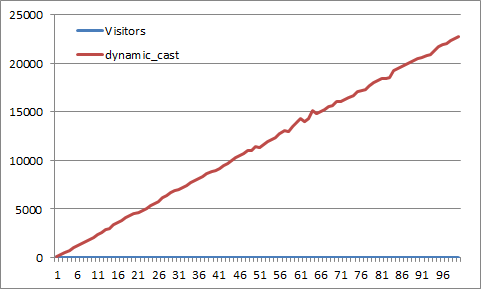
\includegraphics[width=0.47\textwidth]{DCast-vs-Visitors.png}
  \caption{Type switching based on naive techniques}
  \label{fig:DCastVis1}
\end{figure}

The simple scheme of assigning a unique tag per variant (instantiatable class 
here) will not pass our first question because the tags of base and derived 
classes will have to be different if the base class can be instantiated on its 
own. In other words we will not be able to land on a case label of a base class 
having a derived tag only. The already mentioned partitioning of tags of derived 
classes based on the classes in case clauses also will not help as it assumes 
knowledge of all the classes and thus fails extensibility through DLLs.

In practical implementations hand crafted for a specific class hierarchy, tags 
often are not chosen arbitrarily, but to reflect the subtyping relation of the 
underlain hierarchy. Switching on base classes in such setting will typically 
involve a call to some function $f$ that converts derived class' tag into a base 
class' tag. An example of such scheme would be having a certain bit in the tag 
set for all the classes derived from a given base class. Unfortunately this 
solution creates more problems then it solves.

First of all the solution will not be able to recognize an exceptional case 
where most of the derived classes should be handled as base class, while few 
should be handled specifically. Applying function $f$ puts several different 
types into an equivalence class with their base type, making them 
indistinguishable from each other.

Secondly, the assumed structure of tags is likely to make the set of tags 
sparce, effectively forcing compiler to use a decision tree instead of jump 
table to implement the switch. Even though conditional jump is reported to be 
faster than indirect jump on many computer architectures~\cite[\textsection 
4]{garrigue-98}, this did not seem to be the case in our experiments. 

Besides, as was seen on the scheme of Gibbs and Stroustrup, the assumed 
structure of tags can also significantly decrease the amount of classes a given 
allocation scheme can handle.

Summarizing, truly open and efficient type switching seems to be a non trivial 
problem. The implementations we found in the literature where either open or 
efficient, but not both. Efficient implementation was typically achieved by 
sealing class hiearchy and using jump table. Without sealing, the implementation 
was resorting to decision trees and type testing, which was not efficient.
We are unaware of any efficient tag allocation scheme that can be used in a 
truly open scenario.

\section{Related Work} %%%%%%%%%%%%%%%%%%%%%%%%%%%%%%%%%%%%%%%%%%%%%%%%%%%%%%%%%
\label{sec:rw}

A solution to extensibility of visitors with new classes has been proposed in the form of \emph{Extensible 
Visitors with Default Cases}\cite[\textsection 4.2]{Zenger:2001}, however the solution, after 
remapping it onto C++, has problems of its own. The visitation interface 
hierarchy can easily be grown linearly (adding new cases for the new classes in 
the original hierarchy each time), but independent extensions by different  
authorities require developer's intervention to unify them all, before they can 
be used together. This may not be feasible in environments that use dynamic 
linking. To avoid writing even more boilerplate code in new visitors, the 
solution would require usage of virtual inheritance, which typically has 
an overhead of extra memory dereferencing. On top of the double dispatch already 
present in the visitor pattern, the solution will incur two additional virtual 
calls and a dynamic cast for each level of visitor extension. Additional double 
dispatch is incurred by forwarding of default handling from base visitor to a 
derived one, while the dynamic cast is required for safety and can be replaced 
with a static case when visitation interface is guaranteed to be grown linearly 
(extended by one authority only). Yet another virtual call is required to be 
able to forward computations to subcomponents on tree-like structures to the 
most derived visitor. This last function lets one avoid the necessity of using 
heap to allocate a temporary visitor through the \emph{Factory Design 
Pattern}\cite{DesignPatterns1993} used in \emph{Extensible Visitor} solution 
originally proposed by Krishnamurti, Felleisen and Friedman\cite{Krishnamurthi98}.

There are two main approaches to compiling pattern matching code: the first is 
based on \emph{backtracking automata} and was introduced by Augustsson\cite{}, 
the second is based on \emph{decision trees} and is attributed in the literature 
to Dave MacQueen and Gilles Kahn in their implementation of Hope compiler \cite{}.
Backtracking approach usually generates smaller code, while decision tree 
approach produces faster code by ensuring that each primitive test is only 
performed once. Neither of the approaches addresses specifically type patterns 
or type switching and simply assumes presence of a primitive operation capable 
of performing type tests.

In order to address expression problem in Haskell, L\"{o}h and Hinze proposed to 
extend its type system with open data types and open functions\cite{LohHinze2006}.
Their solution allows the user to mark top-level data types and functions as 
open and then provide concrete variants and overloads anywhere in the program. 
The semantics of open extension is given by transformation into a single module, 
where all the definitions are seen in one place. While open data types introduce 
some of the problems that subclassing does in object-oriented languages, the 
problems are simpler. As we discussed before, the object-oriented analog of 
adding new variants is addition of a class that implements a given interface. In 
other words it is a derived class that extends a strictly flat class hierarchy. 
This largely avoids the problem of classes having multiple types and thus the 
problem of type switching on base classes. Another limitation of their approach 
that prevents from calling it a truly open solution is the fact that their 
semantics essentially assumes a whole program view, which excludes any 
extensions via DLLs. As is the case with many other implementations of open 
extensions authors rely on the closed world for efficient implementation: in 
their implementation \emph{data types can only be entirely abstract (not 
allowing pattern matching) or concrete with all constructors with the reason 
being that pattern matching can be compiled more efficiently if the layout of 
the data type is known completely}. The authors also believe that \emph{there 
are no theoretical difficulties in lifting this restriction, but it might imply 
a small performance loss if closed functions pattern match on open data types}. 

\bibliographystyle{abbrvnat}
\bibliography{mlpatmat}
\end{document}
